%!TEX program = xelatex
% 完整编译方法 1 pdflatex -> bibtex -> pdflatex -> pdflatex
% 完整编译方法 2: xelatex -> bibtex -> xelatex -> xelatex
\documentclass[lang=cn,11pt]{elegantpaper}
\usepackage[T1]{fontenc}
\usepackage{mathtools}    % loads »amsmath«

\title{电磁法在地热勘探中的应用}
\author{杨 建 熙}

\institute{\href{https://elegantlatex.org/}{Elegant\LaTeX{} 项目组}}

% 不需要版本信息,直接注释即可
\version{0.07}
% 不需要时间信息的话,需要把 \today 删除。
\date{\today}


% 如果想修改参考文献样式,请把这行注释掉
\usepackage[authoryear]{gbt7714}  % 国标

\begin{document}

\maketitle

\begin{abstract}
\noindent 地热资源作为一种清洁能源,具有绿色环保可持续的特性,有别于传统的石油天然气,存在巨大的开发潜力,将会在我国未来的经济发展中起到巨大的作用。而地热资源的勘探,是开发利用地热资源的前提,地热资源的勘探是地热资源开发和利用的基础,也是地球物理方法重要的应用领域。地球物理方法应用于地热探测具有悠久的历史,形成了一套较完备的探测方法技术和数据处理和解释方法。包括航空、地面和井中地球物理方法,而电磁法在地热勘探中应用广泛,本文主要通过查阅文献,结合实例讨论如何使用电磁法寻找地热资源。
\end{abstract}


\section{电磁法原理}
电磁感应法是以地壳中岩石和矿石的的导电性与导磁性差异为主要物质基础,根据电磁感应原理观测和研究电磁场空间与时间分布规律,从而寻找地下良导体的一组分支电法勘探方法,简称电磁法。

 \begin{subequations}
     \begin{alignat}{2}
        \mathllap{\text{高斯定理}\qquad} && \nabla \times \emph{\textbf{H}} &=\sigma \emph{\textbf{E}} + \varepsilon   \frac{\partial\emph{\textbf{E}}}{\partial t} \\
        \mathllap{\text{高斯定理}\qquad} && \nabla \times \emph{\textbf{E}} &=-\mu  \frac{\partial\emph{\textbf{H}}}{\partial t} \\
        \mathllap{\text{法拉第定律}\qquad} && \nabla \cdot \emph{\textbf{H}} &=0 \\
        \mathllap{\text{安培定理}\qquad} && \nabla \cdot \emph{\textbf{E}} &=0
     \end{alignat}
   \end{subequations}


\begin{figure}[htbp]
	\centering
	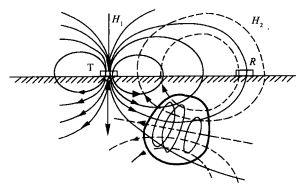
\includegraphics[width=0.6\textwidth]{ele.png}
	\caption{电磁感应原理图 \label{fig:scatter}}
\end{figure}

常用的电磁法有大地电磁法,可控源音频大地电磁法以及瞬变电磁法。大地电磁测深法(MT),是通过改变电磁场的频率进行测深的一类电法分支,它利用电磁感应的趋肤效应,即高频电磁场穿透浅,低频电磁场穿透深,在场源和接收点间距不变的条件下,改变电磁场的频率来达到测深的目的。MT法对深部构造有较高的分辨率。
可控源音频大地电磁法(CSAMT)是在大地电磁法和音频大地电磁法(AMT)上发展起来的一种人工源频率域测深方法,采用人工场源供电,频率范围为0.25 ~ 8192Hz。可控源音频大地电磁测深是以有限长接地导线为场源,在距场源中心一定距离处同时观测电、磁场参数的一种电磁测深方法。目前应用大多采CSAMT法所观测的电磁场频率范围、场强和方向可由人工控制,观测方法与MT方法相同。CSAMT法抗干扰能力强,对浅部不均匀体有较细的刻画。目前应用大多采用赤道偶极装置进行标量测量,同时观测与场源平行的电场水平分量
,和与场源正交的磁场水平分量  。利用电场振幅 和磁场振幅 计算卡尼亚视电阻率$\rho_s$

\section{地热勘探的基本原理}
地热勘探的地球物理方法有许多种,重力方法,磁法,地震方法,钻探,以及电法,地温探测法。由于地下热水能够使岩层电阻率降低,所以以往地热资源调查中,直流电阻率法一直占主导地位。但是随着地热资源开发的深度越来越大,大多已经超过了2000米,地表观测到由地热异常引起的电阻率差异越来越小,而近几年来,我们采用可控源音频大地电磁测深法(CSAMT),分别在北京、辽宁、河北和浙江等地进行了深部地热资源调查,取得了较好的地质效果。
电性参数是地球物理电法,电磁法勘探中最重要的参数,也是应用于地热勘查最重要的方法基础,电阻率在地热的勘查中作用非常明显,一方面,构造带、地热田的生储盖等不同部位具有较明显的电性差异.对于构造带型的热储,其电阻率与围岩电阻率的差异在很多文献中讨论过另一方面,随着温变的升高,电阻率发生很大的变化,这也是电法和电磁法在地热勘查中作用明显的另一个重要原因。
地下的热作用,将很明显改变岩石的地球物理性质,地热区电阻率的空间分布不仅受围岩性质的影响,还与勘探对象一热水的分布直接有关.前苏联科学家T.A.Dakhnow通过大量试验研究,得出含水岩层电阻率和温度变化之间的关系为
地下的热作用,将很明显改变岩石的地球物理生质,地热区电阻率的空间分布不仅受围岩性质的影响,还与勘探对象一热水的分布直接有关,前苏联科学家T.A.Dakhnow通过大量试验研究,得出含水岩层电阻率和温度变化之间的关系为\\
式中, , 分别是地层温度为20℃和t℃时的地层电阻率,α是岩石温度系数,岩石温度系数和岩性及含水溶液矿化度有关。	
由于水热系统的存在,除了温度和热流的升高以外,也许最重要的物理性质是改变是岩流体积的电阻率变化,大概直到300℃,温度升高使离子的迁移率增加,因此使电导率增加而增加。总体上,随着温度的升高,低。可见在地热田勘查中,低阻标,由于它的直接指示作用和地差异明显,电法和电磁法也就成最直接有效的方法技术。


\section{案例分析——开封凹陷地热资源调查(MT法)}
    \subsection{电性特征}
    第四系主要为砂、黏土,电阻率一般为低阻,总体上表现为电性不均,一般电阻率为8~ 19Ψ•m。新近系分为明化镇组和馆陶组,电阻率为4~13Ψ•m。明化镇组与第四系之间的电性界线并不清楚,跟馆陶组电性差异也极小,很难单独划分出一层来,故以Q-Ng来代表第四系到馆陶组。古近系以砂岩、泥岩为主,古近系电阻率表现为低阻,一般为2~ 5Ψ•m。总之,本区各时代的地层由于沉积环境及地质环境的不同,在电性上有一定的差异。尤其是基底电阻率值,从MT测深成果看一般在20~ 40Ψ•m,远远低于区域上同类岩石电阻率,预示着本区有良好的地热富集前景。根据MT测深结果,结合区域地质资料,古近系为低阻,故定为电性标志层。图1为区内较典型的MT视电阻率曲线,可见在0.04Hz左右有一明显的低阻反映(H型曲线段),此为古近系的反映。

     \begin{figure}[htbp]
	\centering
	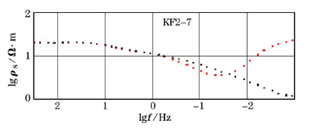
\includegraphics[width=0.6\textwidth]{dzl.png}
    \caption{电磁感应原理图 \label{fig:scatter}}
    \end{figure}

     \subsection{工作布置}

     \begin{figure}[htbp]
	\centering
	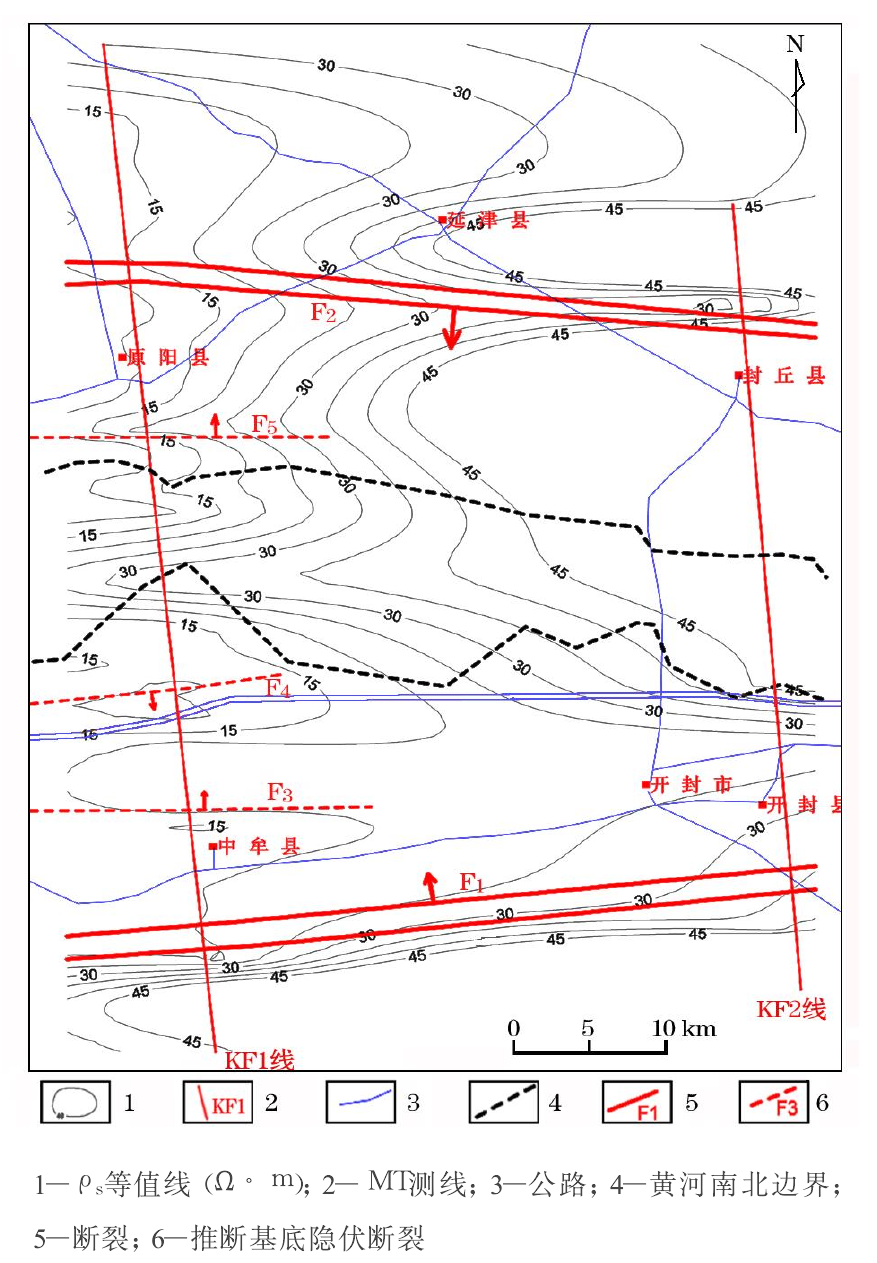
\includegraphics[width=0.6\textwidth]{ghbz.png}
     \caption{电磁感应原理图 \label{fig:scatter}}
    \end{figure}

     工作中采用具有GPS同步功能的V52000MT系统实施野外数据采集。M野外数据采集时间不少于6h以保证数据量及探测深度和质量。数据采集采用1:8:5方式。电极采用Pb-Pbc12不极化电极,其具有低噪音、低漂移等特点。测地工作使用GPS GARIN 小博士全球卫星定位仪。工区内共布置MT测线2条,相距40lm设计测点50个图2),其中,K1线上的5B5C为补测点。每个测深点采集时间为7~10h最长达到13
     b每个测深点采集38或40个频率,频率范围为320~0.000549H有效勘探深度大于3lnd2l。

     \subsection{成果解释}
     MT解释的地热异常区仍以高阻基底地层为背景,因为地热水为低阻表现,电法只能从高阻的背景中找低阻。从测量结果看,高阻基底大部分测点电阻率值小于45Ψ•m,出现明显的电性异常现象。这说明测区内受地热影响而导致地球物理场变化的现象是客观存在的,这也是我们研究高阻基底热储、划分其地热富集分布范围的基本依据。可根据高阻基底的电性变化,圈定本区地热异常范围,即在平面上大致以高阻基底电阻率值小于45Ψ•m等值线为界,圈出了主要异常区(图6)。异常区主要分布在F1 断裂以北大部地区,即KF1线的4~ 39点,KF2线的2~ 5、9、11点。

      \begin{figure}[htbp]
	\centering
	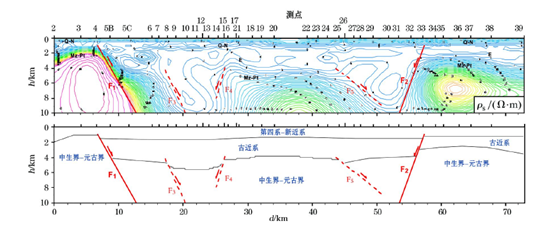
\includegraphics[width=1.0\textwidth]{cg.png}
    \caption{$KF_1$线二维连续介质反演剖面及地质推断 \label{fig:scatter}}
    \end{figure}

\section{结论与建议}
地热资源是一种新能源,绿色环保,可持续发展,地热资源的用途广泛,传统的发电方式主要是火力发电,需要燃烧化石燃料,而化石燃料的燃烧会释放二氧化碳等污染物,会严重影响空气质量,对空气造成污染。风力发电和太阳能发电往往成本过高,受到天气影响严重,而地热发电直接利用地下的热量,基本上取之不尽用之不竭,而且真正能做到清洁无污染。但是目前人们对于地热资源的利用率还不高,还处在探索阶段,深部的资源开采和利用和开采还需要技术的改进,所以对地热的研究是非常有必要的,在将来地热势必会成为人类生活中必不可少的资源。
地热资源的勘探,方法有许多种,但是最主要的方法还是地球物理方法,而地球物理方法本身为了研究和寻找固体矿物的勘探方法,但是也可以根据地下介质的波速、重力、磁异常,以及放射性,电性等特征来寻找地热资源,而且,效果良好,另一方面,地球物理方法依旧可以用在工程建筑、地基勘查等方面。可见任何一种方法都是灵活多变的,不能把地球物理方法局限在某一特定领域。
另外一方面,地热资源的勘探目前主要还是依据地球物理方法,但是却没有一种专门用于地热勘探,专门针对地热资源,专门利用地温特性的方法来寻找地热资源。这样就会造成许多误判,需要做更多的分析,来分析和判断,到底异常体是由于什么原因产生的,因此我们缺少一种能一次性做出判断的方法。
地热资源根据地温梯度的变化规律,越往地下越深,温度也越高,因此一般的地球物理方法效果就变得不明显,也正是因此,所以电磁法才显出优势,因为电磁法的勘探深度相较于其他电法,勘探深度也越深,然而,随着勘探深度的增加,电磁波的衰减也就越严重,得到的数据误差也越大,反演也变得困难。因此地球物理方法的发展方向还是要往深处,往精细发展。
众所周知,红外线对温度比较敏感,我们是否可以充分利用更多跟温度有关的特性来寻找地热资源,如何实现深部热红外成像,如何根据地下放射性特征来判断地热资源,是否可以类似的像使用电场一样来研究温度场,并最终实现地热资源勘探,我觉得,这是我们考虑的。

\section{参考文献}
\nocite {*}
\bibliography{direkantan}
\section{模板介绍}
此模板是基于 \LaTeX{} 的标准文类 article设计,也即意味着你可以把 article 文类的选项传递给本模板,比如 \lstinline{a4paper, 10pt} 等等(推荐使用 \lstinline{11pt})。本模板支持 \lstinline{PDFLaTeX} 和 \lstinline{XeLaTeX}\footnote{中文字体均使用 \lstinline{ctex} 包设置。} 两种编译方式。

数学字体的效果如下:

\begin{equation}
(a+3b)^{n} = \sum_{k=0}^{n} C_{n}^{k} a^{n-k} (3b)^k\label{eq:binom}
\end{equation}

\subsection{全局选项}
我在这个模板中定义了一个语言选项 \lstinline{lang},可以选择英文模式 \lstinline{lang=en}(默认)或者中文模式 \lstinline{lang=cn}。当选择中文模式时,图表的标题引导词以及参考文献,定理引导词等信息会变成中文。你可以通过下面两种方式来选择语言模式:

\begin{lstlisting}
\documentclass[lang=cn]{elegantpaper} % or
\documentclass{cn}{elegantpaper}
\end{lstlisting}


\subsection{自定义命令}
在此模板中,并没有修改任何默认的命令或者环境,所以,你可以在此模板使用原来的命令和环境。另外,我自定义了 3 个命令:

\begin{enumerate}
	\item \lstinline{\email}:创建邮箱地址的链接;
	\item \lstinline{\figref}:用法和 \lstinline{\ref} 类似,但是会在插图的标题前添加 <\textbf{图 n}> ;
	\item \lstinline{\tabref}:用法和 \lstinline{\ref} 类似,但是会在表格的标题前添加 <\textbf{表 n}>;
	\item \lstinline{\keywords}:为摘要环境添加关键词。
\end{enumerate}



\subsection{列表环境}
你可以使用列表环境(\lstinline{itemize}、\lstinline{enumerate}、\lstinline{description}),示例如下:\\[2ex]
\begin{minipage}[c]{0.59\linewidth}
\begin{lstlisting}
\begin{itemize}
   \item Routing and resource discovery;
   \item Resilient and scalable networks;
   \item Distributed storage and search.
\end{itemize}
\end{lstlisting}
\end{minipage}
\begin{minipage}[c]{0.4\linewidth}
\begin{itemize}
   \item Routing and resource discovery;
   \item Resilient and scalable networks;
   \item Distributed storage and search.
\end{itemize}
\end{minipage}




\subsection{插图}
插图的命令和以前一样,也是使用 \lstinline{figure} 环境。\figref{fig:scatter} 显示了插图的效果。你可以把你的图放到当前工作目录的如下子目录下 (\lstinline{./image/}, \lstinline{./img/}, \lstinline{./figure/}, \lstinline{./fig/})。


\begin{lstlisting}
\begin{figure}[htbp]
	\centering
	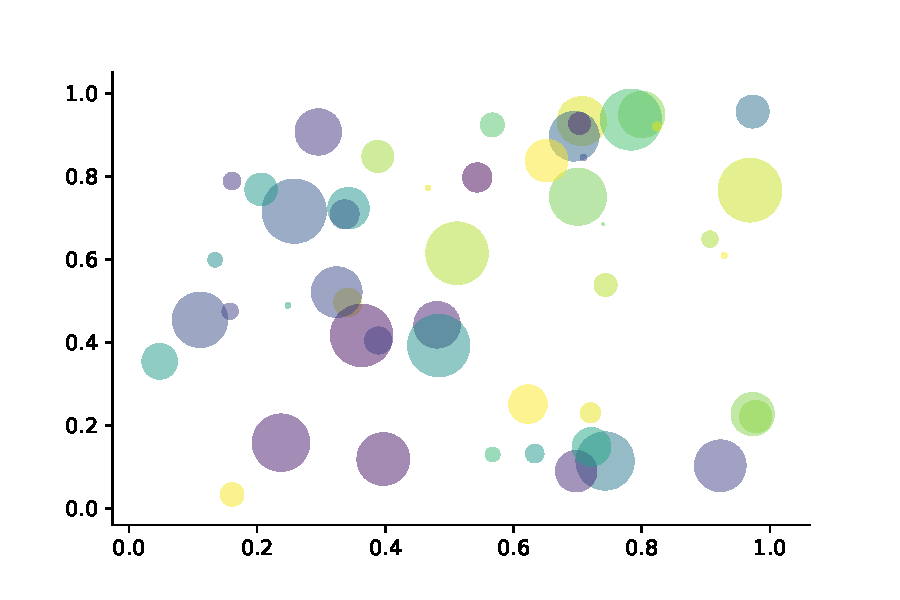
\includegraphics[width=0.6\textwidth]{scatter.pdf}
	\caption{Scatter Plot Example \label{fig:scatter}}
\end{figure}
\end{lstlisting}
\begin{figure}[htbp]
	\centering
	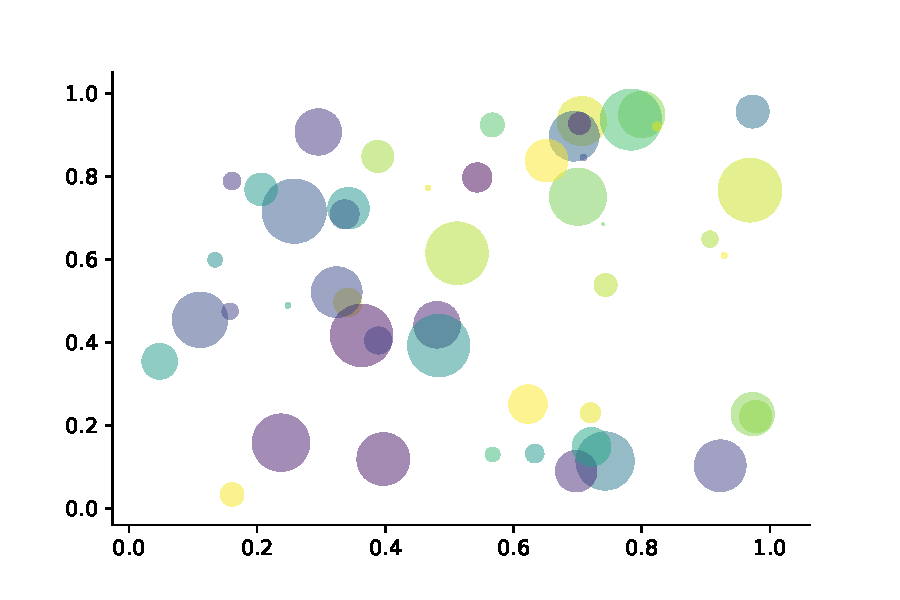
\includegraphics[width=0.6\textwidth]{scatter.pdf}
	\caption{Scatter Plot Example \label{fig:scatter}}
\end{figure}

\subsection{表格}
我强烈建议你使用 \lstinline{booktabs} 宏包,这个宏包有三个命令 \lstinline{\toprule}、\lstinline{\midrule} 和 \lstinline{\bottomrule} 能方便你制作三线表。\tabref{tab:reg} 是一个示例:

\begin{lstlisting}
\begin{table}[htbp]
  \small
  \centering
  \caption{Auto MPG and Price \label{tab:reg}}
    \begin{tabular}{lcc}
    \toprule
                    &       (1)         &        (2)      \\
    \midrule
    mpg             &    -238.90***     &      -49.51     \\
                    &     (53.08)       &      (86.16)    \\
    weight          &                   &      1.75***    \\
                    &                   &      (0.641)    \\
    constant        &     11,253***     &       1,946     \\
                    &     (1,171)       &      (3,597)    \\
    obs             &        74         &         74      \\
    $R^2$           &      0.220        &       0.293     \\
    \bottomrule
    \multicolumn{3}{l}{\scriptsize Standard errors in parentheses} \\
    \multicolumn{3}{l}{\scriptsize *** p<0.01, ** p<0.05, * p<0.1} \\
    \end{tabular}%
\end{table}%
\end{lstlisting}
\begin{table}[htbp]
  \small
  \centering
  \caption{Auto MPG and Price \label{tab:reg}}
    \begin{tabular}{lcc}
    \toprule
                    &       (1)         &        (2)      \\
    \midrule
    mpg             &    -238.90***     &      -49.51     \\
                    &     (53.08)       &      (86.16)    \\
    weight          &                   &      1.75***    \\
                    &                   &      (0.641)    \\
    constant        &     11,253***     &       1,946     \\
                    &     (1,171)       &      (3,597)   \\
    obs             &        74         &         74     \\
    $R^2$           &      0.220        &       0.293    \\
    \bottomrule
    \multicolumn{3}{l}{\scriptsize Standard errors in parentheses} \\
    \multicolumn{3}{l}{\scriptsize *** p<0.01, ** p<0.05, * p<0.1} \\
    \end{tabular}%
\end{table}%



\subsection{参考文献}
此模板使用了 Bib\TeX{} 来生成参考文献,默认使用的文献样式(bib style)是 \lstinline{GB/T 7714-2015}\footnote{通过调用 \href{https://ctan.org/pkg/gbt7714}{\lstinline{gbt7714}} 宏包}。参考文献示例:~\cite{en3} 使用了中国一个大型的 P2P 平台(人人贷)的数据来检验男性投资者和女性投资者在投资表现上是否有显著差异。

你可以在谷歌学术,Mendeley,Endnote 中获得文献条目(bib item),然后把它们添加到 \lstinline{wpref.bib} 中。在文中引用的时候,引用它们的键值(bib key)即可。注意需要在编译的过程中添加 Bib\TeX{} 编译。如果你想在参考文献中添加未引用的文献(部分或者全部),可以使用

\begin{lstlisting}
\nocite{EINAV2010, Havrylchyk2018} % add the two reference.
\nocite{*}   % add all the reference in the bib file.
\end{lstlisting}

如果你想修改参考文献的样式(比如改为 \lstinline{aer}),你可以在导言区将下面代码注释掉。
\begin{lstlisting}
\usepackage[authoryear]{gbt7714}
\end{lstlisting}

并且文档末尾添加

\begin{lstlisting}
\bibliographystyle{aer}
\end{lstlisting}

\section{示例}
在这部分,我提供一个示例文档:


\begin{lstlisting}
\documentclass[lang=cn]{elegantpaper}

% title information
\title{A Working Paper Example}
\author{ddswhu}
\institute{Elegant\LaTeX{} Group}
\version{1.00}
\date{\today}

\begin{document}

\maketitle

\begin{abstract}
Your abstract goes here.
\keywords{keyword1, keyword2}
\end{abstract}

\section{Introduction}
The content of introduction section.

\section{Conclusion}
The content of conclusion section.

% include the noncited reference
\nocite{ref1, ref2}
\bibliographystyle{aer}
\bibliography{wpref}
\end{document}
\end{lstlisting}

\nocite{*}

% 如果想修改参考文献样式(非国标),请把下行取消注释,并换成合适的样式(比如 unsrt,plain 样式)。
%\bibliographystyle{aer}
\bibliography{wpref}

\end{document}
